% paper.tex — HPCC-FS submission skeleton (ACM acmart conference template).
% Compile: pdflatex paper && bibtex paper && pdflatex paper && pdflatex paper
% Companion file: paper.bib

\documentclass[sigconf, nonacm]{acmart}

\settopmatter{printacmref=false}
\renewcommand\footnotetextcopyrightpermission[1]{}
\pagestyle{plain}

\usepackage{booktabs}
\usepackage{graphicx}
\usepackage{xcolor}
\usepackage{listings}
\usepackage{microtype}
\usepackage{url}
\usepackage{amsmath}
\usepackage{algorithm}
\usepackage{algpseudocode}

\graphicspath{{figures/}}

% Convenience macros
\newcommand{\hpccfs}{\textsc{HPCC-FS}\xspace}
\usepackage{xspace}

\title[HPCC-FS: Multi-Bottleneck Fairness]{Multi-Bottleneck Fairness for High-Precision Congestion Control}

\subtitle{A Minimal Switch Extension for Multi-Bottleneck Max-Min Fairness}

\author{Haoyu Wang}
\affiliation{%
  \institution{University of Massachusetts Boston}
  \city{Boston}
  \state{MA}
  \country{USA}}
\email{haoyu.wang001@umb.edu}

\author{Bo Sheng}
\affiliation{%
  \institution{University of Massachusetts Boston}
  \city{Boston}
  \state{MA}
  \country{USA}}
\email{bo.sheng@umb.edu}

\author{Zerin Shaima Meem}
\affiliation{%
  \institution{University of Nebraska Omaha}
  \city{Omaha}
  \state{NE}
  \country{USA}}
\email{zmeem@unomaha.edu}

\author{Xiaoqian Zhang}
\affiliation{%
  \institution{University of Nebraska Omaha}
  \city{Omaha}
  \state{NE}
  \country{USA}}
\email{xiaoqianzhang@unomaha.edu}

\begin{abstract}
HPCC (SIGCOMM '19) achieves near-optimal flow completion time for single-bottleneck RDMA
workloads via INT-based precision congestion control with no per-flow switch state. We show its
design has a structural fairness failure on \emph{multi-bottleneck} paths --- increasingly common
in cross-pod and disaggregated datacenter traffic: a flow crossing several shared bottlenecks is
starved by ${\sim}2\times$ relative to single-bottleneck competitors, and fails entirely once the
per-hop INT record overflows its hop budget. Through a five-variant sender-side ablation we show
the gap is not closable from the endpoint --- a sender cannot compute its max-min fair share
because the link's flow count is not observable in INT. The fix belongs at the switch. \hpccfs
adds a single RCP-style fair-rate signal --- one 64-bit header field and one scalar of state per
egress port --- whose fixed point is the max-min share, reached \emph{without ever counting flows}.
It drives the multi-bottleneck penalty to ${\approx}1.0\times$ across bottleneck counts, asymmetric
flow sizes, staggered starts, and ECMP fat-trees, with zero PFC. We are explicit that the mechanism
is RCP; our primary contribution is the \emph{diagnosis} and the demonstration that the fix belongs
in the network, not the endpoint. The stock HPCC code path is left byte-for-byte unchanged.
\end{abstract}

\begin{document}

\maketitle

% ============================================================================
\section{Introduction}
% ============================================================================

HPCC~\cite{li2019hpcc} and its derivatives represent the state of the art in datacenter RDMA
congestion control. Their design philosophy is unusually clean: the switch stamps raw per-hop
state (transmitted bytes, queue length, link rate) into INT headers; the sender computes a
precise utilization estimate and applies a multiplicative-increase, multiplicative-decrease
update toward a target utilization $\eta$. The switch is stateless per flow; the wire format
adds only a few bytes per hop; and on the canonical single-bottleneck benchmarks HPCC matches
or beats DCQCN, TIMELY, and DCTCP on flow completion time and queueing.

Modern datacenter workloads, however, increasingly involve traffic that traverses
\emph{multiple contended links} in series: cross-pod ML allreduce, disaggregated memory and
storage, and multi-tenant flows that share aggregation and core layers. Whether HPCC's design
still delivers fair, low-latency service in these settings has not been carefully measured.

We address that question with a deterministic, oracle-grounded methodology. Our contributions:

\begin{enumerate}
\item \textbf{An empirical characterization} of HPCC's multi-bottleneck behaviour using a
parameterized parking-lot benchmark and a fluid max-min oracle (\S\ref{sec:bg}). We show the
multi-bottleneck penalty is real (${\sim}1.9\times$ at $N = 2$--$4$), worse for small flows
($3.5\times$), robust to flow-size asymmetry and start staggering, and \emph{RTT-independent}:
equalizing the long flow's RTT with the cross flows' does not move the penalty.

\item \textbf{A negative result for sender-only fixes} (\S\ref{sec:senderonly}). We implement
five sender-side variants of HPCC ranging from a $k$-aware additive boost to a global
share-aware update rule, and show all five fail to close the gap. We give a structural
explanation: at the multi-bottleneck equilibrium every flow holds its current rate (because
the bottleneck utilization sits at $\eta$, making the multiplicative term ${\approx}1$), and
a sender cannot compute the strong multiplicative correction needed without knowing the link's
flow count $N$.

\item \hpccfs, \textbf{a switch-minimal design that instantiates the fix with RCP-style control}
(\S\ref{sec:design}). On contended flows \hpccfs does \emph{not} use HPCC's per-hop, window-bounded
control law; instead each switch port runs a standard RCP~\cite{dukkipati2008rcp} fair-rate update
on aggregate load and queue, advertises that single rate in the INT header, and the sender adopts
the path-minimum. The switch addition is minimal --- one uint64 field in a new INT header mode and
one scalar of state per egress port --- which is where prior INT-based designs spend their
complexity; the full deployment delta is slightly larger (a new sender ACK handler, and, in our
prototype, rate-only operation with the per-flow window cap disabled). We are explicit that the
mechanism is RCP, not a new control law: our contribution is showing that placing this signal at
the switch is what closes the gap, and that doing so is cheap and leaves the existing HPCC code
path (\texttt{cc\_mode 3}) byte-for-byte unchanged.

\item \textbf{An evaluation showing \hpccfs achieves the goal} (\S\ref{sec:eval}): max-min
penalty ${\approx}1.005\times$ at $N=4$, zero PFC events, robust across asymmetric workloads,
generalizing to a tree-fabric and to a $k = 4$ ECMP fat-tree.
\end{enumerate}

Our framing positions the negative result (sender-only designs are insufficient in our
experiments) as a \emph{motivation} for the positive contribution (a minimal switch extension
that suffices on our benchmarks). To our knowledge, this is the first quantitative evidence that
fair-share computation is hard to place purely at the sender in INT-style precision congestion
control; we do not claim a formal impossibility (see Section~\ref{sec:senderonly}).

\paragraph{Artifacts.} The implementation, the topology/workload generators, the max-min oracle,
and deterministic scripts that regenerate the figures (\texttt{make\_figures.py}) and the
ablation/sensitivity/baseline tables (\texttt{run\_sensitivity.py}) from source are available at
\url{https://github.com/UNO-Networks-Lab/uno-hpcc/tree/paper-hpcc-fs/examples/hpcc/hpcc-fs}.

% ============================================================================
\section{Background and Motivation}
\label{sec:bg}
% ============================================================================

\subsection{HPCC, briefly}

HPCC's per-hop utilization estimate for hop $i$ is
\begin{equation}
u_i = \frac{\mathit{txRate}_i}{C_i} + \frac{\min(\mathit{qlen}_i, \mathit{qlen}_i^{\mathrm{prev}}) \cdot \mathit{maxRate}}{C_i \cdot W}
\end{equation}
where the first term reflects bandwidth utilization and the second is a queue-drain term that
keeps standing queues bounded. In single-rate mode the sender takes $U = \max_i u_i$, smooths
it over the base RTT, and applies
\[
\mathit{new\_rate} = \begin{cases} \mathit{curRate} / \max c + R_{AI} & \max c \ge 1 \\ \mathit{curRate} + R_{AI} & \text{otherwise} \end{cases}
\]
with $\max c = U / \eta$. The window $W$ is sized to $m_{win} \cdot \mathit{rate} / \mathit{NIC\_line}$
under \texttt{var\_win}.

\subsection{The multi-bottleneck parking lot}

The \emph{parking lot} is a classic congestion-control fairness
benchmark~\cite{bertsekas1992data, katabi2002xcp}. The name is an analogy: a long boulevard (the
long flow's path) is crossed by a series of side streets, and at each intersection a different
car (a single-link cross flow) merges on and exits. Because every link is equally contended, the
\emph{max-min fair} allocation~\cite{bertsekas1992data} gives every flow an equal share, so the
long flow should run exactly as fast as each cross flow despite traversing many contention points
rather than one. The parking lot therefore isolates the multi-bottleneck fairness question in its
simplest form: any deviation of the long flow's rate from the cross flows' is pure multi-bottleneck
unfairness, with no confounding asymmetry in link capacity or hop count of the competitors.

We construct a parameterized parking-lot benchmark with $N$ inter-switch bottleneck links
(25 Gbps each) and 100 Gbps host links (Figure~\ref{fig:topo-parking}). One ``long'' flow
traverses all $N$ bottlenecks; one ``cross'' flow traverses each single bottleneck. Flows are
50 MB by default and start simultaneously at $t = 0$. With two flows sharing each 25 Gbps link,
the max-min fair rate is 12.5 Gbps for every flow. All experiments are deterministic: each
configuration produces byte-identical artifacts across repeated runs (verified).

\begin{figure*}[t]
\centering
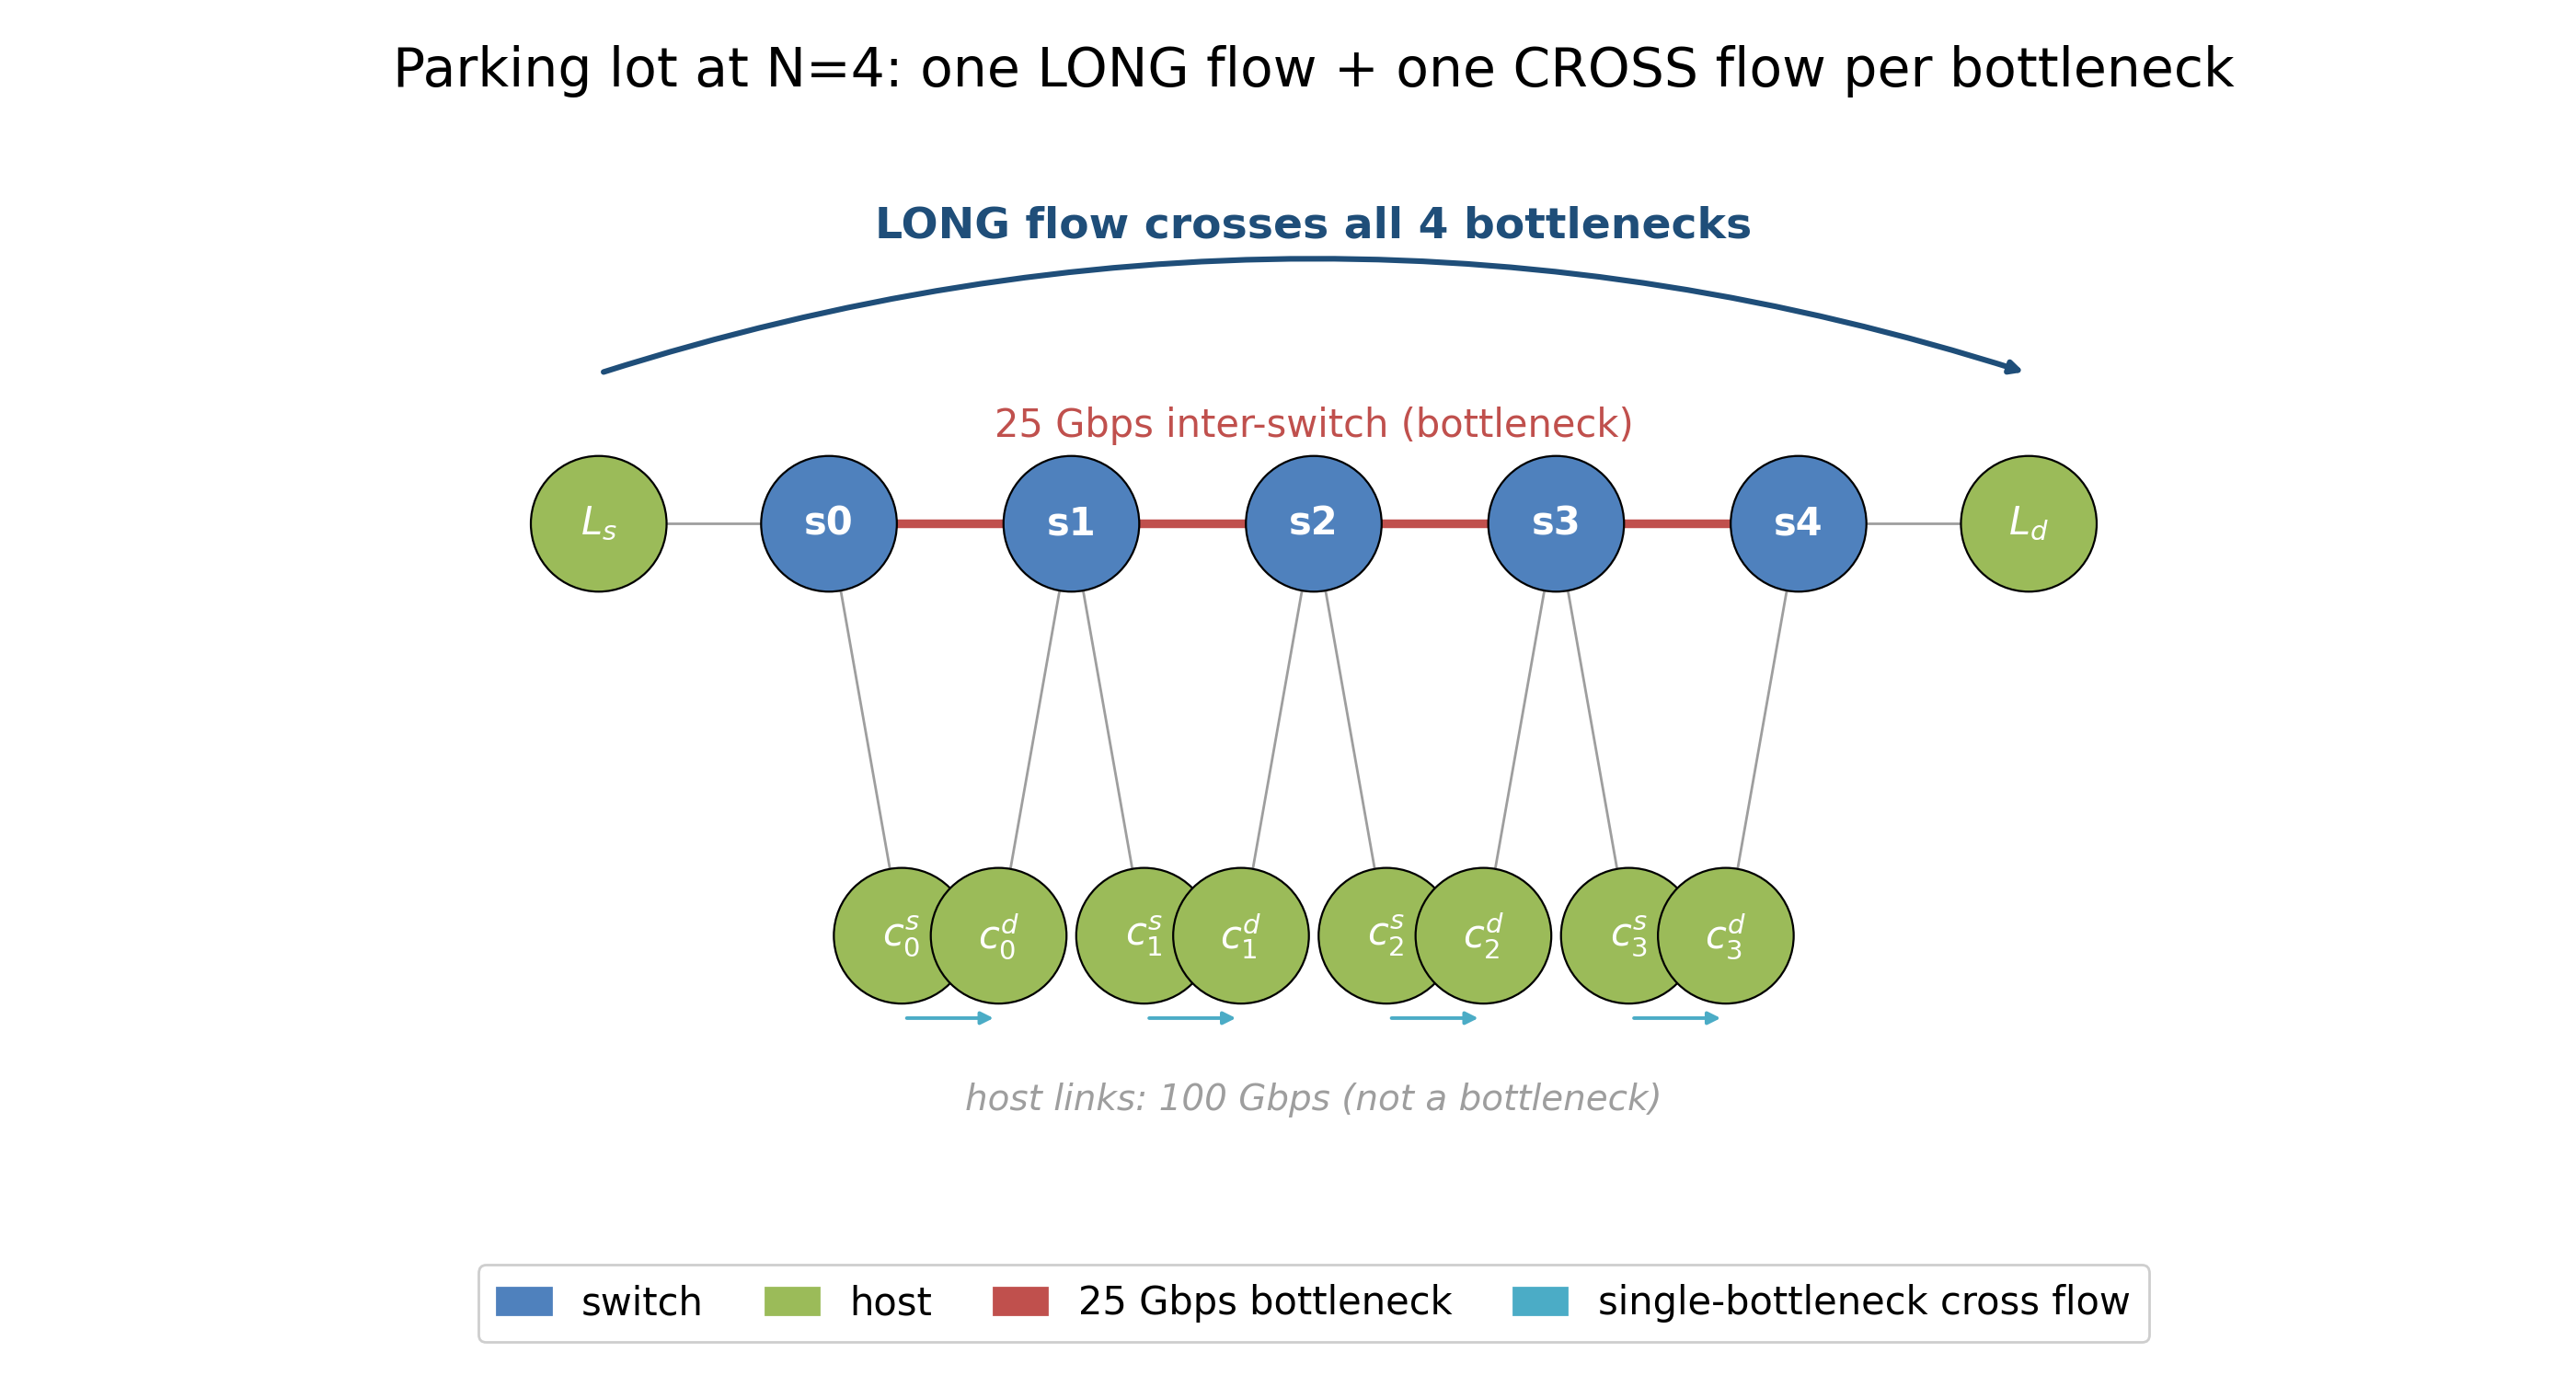
\includegraphics[width=0.92\textwidth]{fig_topo_parking.png}
\caption{Parking-lot benchmark at $N = 4$. The long flow $L_s {\to} L_d$ crosses every
bottleneck; each cross flow $c_i^s {\to} c_i^d$ traverses exactly one. Host links are not
bottlenecks.}
\Description[Parking lot diagram with five switches in a row, four red bottleneck links
between them, host nodes attached, and a curved arrow over the top representing the long
flow that crosses all bottlenecks]{Diagram of the parking-lot topology at N=4: five switches
(s0 to s4) in a horizontal row connected by four thick red 25 Gbps bottleneck links. A long
flow source L_s is attached to s0 and a long flow destination L_d to s4. For each bottleneck
i, two cross-flow hosts (c_i_s under switch i and c_i_d under switch i+1) connect to the
switches below the row via thin gray host links. A curved blue arrow above the switch row
labeled "LONG flow crosses all 4 bottlenecks" indicates the long flow's path. Cross-flow
arrows are shown as short cyan arrows below each bottleneck.}
\label{fig:topo-parking}
\end{figure*}

\paragraph{Metric.} We compare each flow's actual flow completion time (FCT) against an
idealized \textbf{fluid max-min oracle} --- a continuous bandwidth-sharing model with no protocol
dynamics (no slow start, no queueing, no convergence delay) in which the bandwidth is allocated
max-min fairly at every instant. We compute the allocation by \emph{progressive
filling}~\cite{bertsekas1992data}: all active flows raise their rate in lockstep until some link
saturates; the flows crossing that link are frozen at their current rate; and the process repeats
on the remaining flows until every flow is frozen. This is the textbook algorithm for max-min fair
rates. Because flows complete and depart over time, we run it \emph{event-driven} ---
recomputing the allocation at each flow completion --- so the oracle FCT correctly accounts for
the bandwidth freed as short flows finish. The oracle is therefore the best FCT any
rate-allocation scheme could achieve under max-min fairness, and is exact for our fluid
topologies. The headline metric is the \textbf{unfairness ratio}
$\max_{\text{path}}\mathit{FCT} / \mathrm{mean}(\text{short-path FCT})$; the oracle's value is
$1.0$ for equal-size, simultaneous flows.

\subsection{Findings F1--F4: characterizing the gap}

\paragraph{Magnitude.} Stock HPCC's unfairness ratio at $N \in \{2, 3, 4\}$ is $1.90$, $1.92$,
$1.96$: the multi-bottleneck flow's FCT is roughly twice that of single-bottleneck competitors.
\textbf{There is a non-monotonic regime change at $N \ge 5$}, where the long flow becomes
favored ($0.51\times$); this turns out to be an INT-overflow artifact at $\texttt{maxHop} = 5$
and we exclude $N \ge 5$ from the rest of this paper's stock comparisons (Figure~\ref{fig:nsweep}).

\paragraph{Robustness.} Perturbations across flow size and start time give penalties of
$1.81\times$--$3.53\times$ (Figure~\ref{fig:robustness}): stable at $1.8$--$2.0\times$ and
\emph{worsening} dramatically ($3.5\times$) for small multi-bottleneck flows --- the
latency-sensitive RPC / control case. Even an established long flow gets displaced when cross
flows arrive.

\paragraph{HPCC's own multi-rate mode.} Multi-rate HPCC (per-hop EWMA, sender takes
$\min_i Rc_i$) helps but does not fix the gap: $1.44 / 1.50 / 1.75\times$ at $N = 2/3/4$ ---
still growing with bottleneck count.

\paragraph{RTT-equalization rules out RTT unfairness.} Sweeping the bottleneck link delay while
holding $N$ fixed, the penalty is essentially flat at ${\sim}1.9\times$ across cross-flow RTTs
spanning $10\times$ the long flow's RTT (including cases where cross flows have \emph{longer}
RTT than the long flow). The multi-bottleneck penalty is \textbf{not} RTT unfairness.

\paragraph{Trace diagnosis.} A per-flow throughput trace at $N = 4$ (Figure~\ref{fig:rate-trace}
left) shows the qualitative failure: the long flow collapses to ${\sim}0.38$ Gbps while the four
cross flows hold ${\sim}23.2$ Gbps each for the entire 18 ms contention window; only after the
cross flows complete does the long flow take the pipe. There are zero PFC events and zero loss.
The collapse is ``winner-take-all'': at every shared link the single-bottleneck cross flow
wins locally and the long flow is squeezed.

% ============================================================================
\section{Why Sender-Only Fixes Are Insufficient}
\label{sec:senderonly}
% ============================================================================

A natural first design instinct --- and the one our project explored exhaustively --- is to
keep all state and computation at the sender, since HPCC's value proposition is its stateless
switch design. We tried five sender-only correction variants behind a new \texttt{mb\_mode}
config knob, on top of unchanged HPCC. Each is a one- or two-line change in
\texttt{UpdateRateHp}; the \texttt{mb\_mode = 0} path is byte-identical to stock HPCC (verified).

\subsection{The five variants}

\begin{enumerate}
\item \textbf{$k$-aware additive increase} (\texttt{mb\_mode 1}). The flow counts congested hops
$k$ from INT and scales $R_{AI}$ by $\gamma \cdot k$. Result at $N=4$: penalty drops from
$1.96$ to $1.63\times$ at $\gamma = 50$, still nowhere near $1.0$.

\item \textbf{Debiased max/mean blend} (\texttt{mb\_mode 2}).
$U_{\text{eff}} = (1{-}\lambda)\max u_i + \lambda \mathrm{mean}_{u_i \ge \eta} u_i$. Result:
penalty barely moves ($1.95\times$ at $\lambda = 1$), revealing that per-hop $u_i$ are nearly
equal in our setting --- there is no significant max-bias to debias.

\item \textbf{Responsibility-weighted MD} (\texttt{mb\_mode 3}). The flow's multiplicative
decrease is scaled by its measured share $\mathit{own\_rate} / \mathit{txRate}_{\text{btl}}$ at
the bottleneck. Result: $1.89\times$ --- almost no effect, because the MD branch barely fires
at the $\eta$-hold equilibrium.

\item \textbf{$k$-th-root MD} (\texttt{mb\_mode 4}).
$\mathit{new\_rate} = \mathit{curRate} \cdot (1/\max c)^{1/k}$. Result: $1.92\times$.

\item \textbf{Global share-aware additive increase} (\texttt{mb\_mode 5}). Applied to
\emph{every} flow: $R_{AI}^{\mathrm{eff}} = 2(1 - \mathit{share}) \gamma R_{AI}$ when congested.
Result: $1.71\times$ at $\gamma = 20$.
\end{enumerate}

\begin{table}[t]
\caption{Sender-side ablation: best penalty at $N=4$ for each variant.}
\label{tab:ablation}
\centering
\small
\begin{tabular}{rlr}
\toprule
\texttt{mb\_mode} & mechanism & best penalty \\
\midrule
0 & stock HPCC & $1.96\times$ \\
1 & $k$-aware AI ($\gamma=50$) & $1.63\times$ \\
2 & debiased blend ($\lambda=1$) & $1.95\times$ \\
3 & responsibility-weighted MD & $1.89\times$ \\
4 & $k$-th-root MD & $1.92\times$ \\
5 & global share-aware AI ($\gamma=20$) & $1.71\times$ \\
\bottomrule
\end{tabular}
\end{table}

\subsection{The structural reason}

Two observations explain the pattern.

\paragraph{The $\eta$-hold equilibrium.} Once the contended links settle at the target
utilization $\eta$, HPCC's multiplicative term $1/\max c \approx 1$, so the rate update is
dominated by holding. Every flow holds its current rate; if the dominant flows held a high rate
at startup, they keep it. Additive nudges (modes 1, 5) take many tens of thousands of RTTs to
redistribute meaningfully because $R_{AI}$ is small compared to line rate. MD-side
modifications (modes 3, 4) almost never fire because the multiplicative-decrease branch rarely
activates at the hold point.

\paragraph{The information asymmetry.} Strong redistribution requires moving the rate
\emph{multiplicatively} toward each flow's max-min fair share $C / N$. A sender knows $C$ (from
INT) and its own rate, but not $N$ --- the link's flow count. The only $N$-free sender
mechanism is AIMD-style additive nudging, which we have just shown is too slow.

This is precisely why RCP~\cite{dukkipati2008rcp} and XCP~\cite{katabi2002xcp} put the
fair-share computation in the switch. Our results are consistent with the same conclusion for the
HPCC family: across the five representative sender-side designs we evaluated, none converges to the
max-min allocation under the $\eta$-hold dynamics. We present this as empirical evidence, not a
formal impossibility result --- a tight lower bound on what sender-only INT can achieve is left to
future work.

% ============================================================================
\section{HPCC-FS Design}
\label{sec:design}
% ============================================================================

The empirical and structural arguments of \S\ref{sec:senderonly} imply that the fix must (a)
make the \emph{dominant} flows yield, not just nudge the victims, and (b) place a fair-rate
\emph{signal} at the switch, since the sender cannot recover the fair share from a load signal
alone. We do not have the switch count flows and divide; instead it runs a standard RCP control
law on aggregate load and queue (below) whose fixed point \emph{is} the max-min fair rate $C/N$
--- the switch converges to the fair share without ever materializing $N$. We take the most
minimal mechanism consistent with these constraints.

\paragraph{Background: RCP} The Rate Control Protocol (RCP)~\cite{dukkipati2008rcp} is a
router-assisted congestion control in which each link advertises a \emph{single} rate $R$ to
\emph{all} flows crossing it, holding no per-flow state. The key point is that $R$ is not an
aggregate budget for the link; it is the rate \emph{each individual flow} should send at, such
that when all of them do, the link is exactly full and shared equally. A router raises $R$ when
its link has spare capacity and lowers it when a queue forms; routers stamp $R$ into passing
packets, each flow sends at the minimum $R$ along its path, and that rate is echoed to the source.
A single flow adopting $R$ therefore does not seize the link --- it takes its share, because $R$
has already been driven down by the load the other flows place on the same port. Concretely, with
$N$ flows each sending $R$ the offered load is $N R$, and the controller drives $N R \to C$ (idle
link $\Rightarrow$ $R$ rises; standing queue $\Rightarrow$ $R$ falls), so at equilibrium
$R \approx C/N$ --- the max-min (processor-sharing) fair share, tracked \emph{without ever counting
$N$}: as flows arrive or leave, $R$ self-adjusts (a lone flow's $R$ rises to $C$; a third arrival
drops everyone to $C/3$). RCP thus supplies exactly the missing ingredient from
\S\ref{sec:senderonly}: a fair-share signal computed where the flow count is implicitly observable
(the link), not at the sender. HPCC-FS runs this control law once per egress port and carries its
$R$ in the INT header; a flow's path-minimum $R$ yields network-wide max-min fairness, since a
flow bottlenecked elsewhere contributes less load here and the loop hands the slack to the rest.

\subsection{The mechanism}

The entire protocol is Algorithms~\ref{alg:switch} and~\ref{alg:sender}. The switch maintains one
scalar fair rate per egress port and stamps the path-minimum into a single header field; the
sender reads that field from the returning ACK and adopts it. No per-flow switch state, no
per-hop record, no receiver changes.

\begin{algorithm}[t]
\caption{HPCC-FS switch --- per egress port $j$}
\label{alg:switch}
\begin{algorithmic}[1]
\State \textbf{State} $R_j$ (fair rate), $t_j$ (last update), $B_j$ (txByte snapshot)
\State \textbf{Const} $C_j$ link capacity; $\alpha{=}0.4$, $\beta{=}0.226$; $d$ control interval ($\approx$ RTT); $R_{\min}$
\Procedure{OnDequeue}{$pkt$, $j$}\Comment{every packet leaving port $j$}
  \If{$R_j$ uninitialised}
     \State $R_j \gets C_j/2$;\; $t_j \gets now$;\; $B_j \gets \mathit{txBytes}_j$ \Comment{conservative start}
  \EndIf
  \If{$now - t_j \ge d$}\Comment{one control interval elapsed}
     \State $y \gets (\mathit{txBytes}_j - B_j)\cdot 8 \,/\, (now - t_j)$ \Comment{observed load}
     \State $q \gets \mathit{queueBytes}_j \cdot 8$ \Comment{backlog (bits)}
     \State $R_j \gets R_j \cdot \big(1 + (\alpha(C_j - y) - \beta\, q/d)/C_j\big)$ \Comment{RCP update}
     \State $R_j \gets \mathrm{clamp}(R_j,\, R_{\min},\, C_j)$
     \State $t_j \gets now$;\; $B_j \gets \mathit{txBytes}_j$
  \EndIf
  \If{$pkt.\mathit{fairRate} = 0$} \Comment{first hop on the path}
     \State $pkt.\mathit{fairRate} \gets R_j$
  \Else
     \State $pkt.\mathit{fairRate} \gets \min(pkt.\mathit{fairRate},\, R_j)$ \Comment{path-min}
  \EndIf
  \State $\mathit{txBytes}_j \gets \mathit{txBytes}_j + \mathrm{sizeof}(pkt)$
\EndProcedure
\end{algorithmic}
\end{algorithm}

\begin{algorithm}[t]
\caption{HPCC-FS sender (receiver echoes the header unchanged)}
\label{alg:sender}
\begin{algorithmic}[1]
\State \textbf{on} QP-create:\; $\mathit{rate} \gets R_{\min}$ \Comment{conservative start}
\Statex
\Procedure{OnAck}{$a$}
  \If{$a.\mathit{fairRate} = 0$} \Return \Comment{no signal yet}\EndIf
  \State $\mathit{rate} \gets \mathrm{clamp}(a.\mathit{fairRate},\, R_{\min},\, \mathit{NICrate})$ \Comment{adopt path-min fair share}
\EndProcedure
\end{algorithmic}
\end{algorithm}

\paragraph{At the switch (Alg.~\ref{alg:switch}).} Each egress port keeps a single scalar fair
rate $R_j$, refreshed once per control interval $d$ ($\approx$ one RTT) by the standard RCP rule
$R \leftarrow R\,(1 + (\alpha(C - y) - \beta q/d)/C)$, where $y$ is the load observed over the
last interval and $q$ the queue backlog. The term $\alpha(C - y)$ chases spare capacity (positive
while the link is under-utilized, pushing $R$ up) and $\beta q/d$ brakes when a standing queue
forms (pulling $R$ down); they balance at $y \approx C$, $q \approx 0$, which is the
$R \approx C/N$ fixed point above. We use the RCP defaults $\alpha = 0.4$, $\beta = 0.226$
(untuned; the result is insensitive to them, \S\ref{sec:sensitivity}). The port's entire state is
three numbers --- $R_j$, the last update time, and a byte-counter snapshot --- with \emph{no}
per-flow data.

\paragraph{On the wire.} The FS INT mode (\texttt{IntHeader::FS}) carries one 64-bit field,
\texttt{fairRate}; the serialized cost is 8 bytes per packet \emph{independent of hop count}
(vs. 8 bytes \emph{per hop} for stock HPCC). Each switch min-aggregates $R_j$ into this field
(first hop initialises it), so the receiver sees the path-minimum fair rate and echoes the header
back unchanged --- no receiver changes.

\paragraph{At the sender (Alg.~\ref{alg:sender}).} The new ACK handler \texttt{HandleAckFs} reads
\texttt{fairRate} from the returning ACK and sets the sending rate to it, clamped to
$[R_{\min}, \mathit{NICrate}]$. That single assignment is the whole sender control loop.

\subsection{Startup smoothing}

Two cold-start details matter for clean operation. \textbf{Switch:} initialize $R = C/2$ (the
common-case two-flow fair share), not $C$ --- otherwise the first stamped rate is line rate.
\textbf{Sender:} initialize \texttt{qp->m\_rate} to \texttt{m\_minRate} for \texttt{cc\_mode 11},
not the NIC line rate, so the first RTT before any ACK has returned does not blast at line
rate. A flow obtains a path-complete fair-rate signal in a \emph{single} RTT --- unlike stock
HPCC, whose per-link INT estimate needs multiple rounds to reflect a multi-bottleneck path --- but
full convergence to the max-min allocation takes longer, as the per-port RCP estimate settles over
several control intervals (Section~\ref{sec:eval}: ${\sim}4$ ms, i.e. ${\sim}10^2$ RTTs at our
21\,$\mu$s base RTT). HPCC-FS's advantage is therefore \emph{fast, path-length-independent}
convergence, not literal one-RTT convergence.

\subsection{Additive integration}

\hpccfs is \texttt{cc\_mode == 11}. The mode-3 (HPCC) and mode-10 (PINT) wire formats and
switch/sender code paths are completely untouched; we add a fourth case to (a)
\texttt{IntHeader::Mode}, (b) its serialization, (c) the switch's mode-dispatch, (d) the
sender's mode-dispatch, and (e) one branch in the validation driver. The driver also forces the
QP window to 0 in FS mode (rate-only control), since \texttt{var\_win} sizes the window from
the NIC line rate rather than the bottleneck path BDP and would otherwise cap the multi-hop
flow's effective window well below what is needed at its fair rate.

% ============================================================================
\section{Evaluation}
\label{sec:eval}
% ============================================================================

\subsection{Methodology}

All experiments use the deterministic parking-lot benchmark of \S\ref{sec:bg}, driven by our
\texttt{hpcc-validation.cc}. Flows are 50 MB unless noted; sim time is 200 ms; the optimized
binary is used throughout. We compare against stock HPCC (\texttt{cc\_mode 3},
\texttt{multi\_rate = false}), stock HPCC multi-rate, and the \texttt{mb\_mode} ablation suite.

\subsection{Headline: N-sweep}

\begin{figure}[t]
\centering
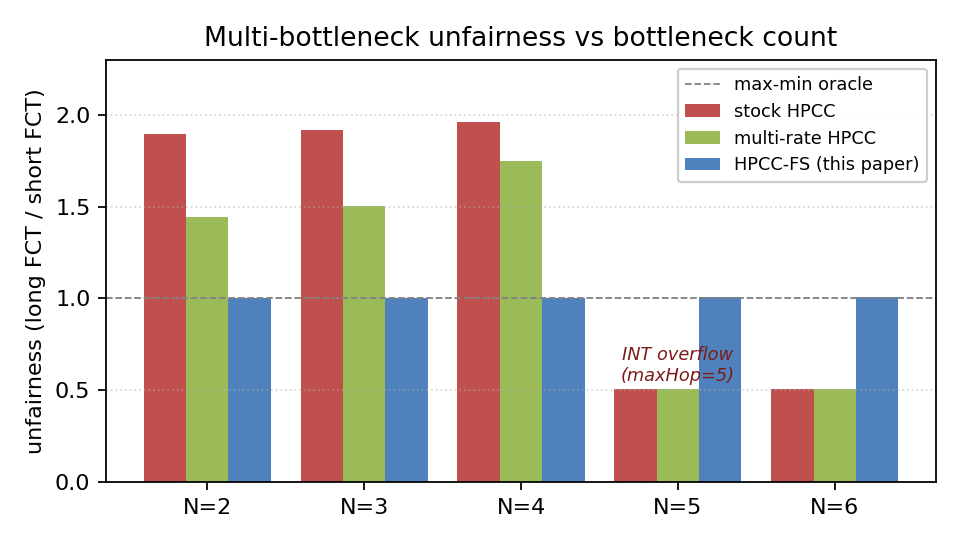
\includegraphics[width=\columnwidth]{fig_nsweep.png}
\caption{Multi-bottleneck unfairness vs bottleneck count $N$. \hpccfs is flat $\approx 1.0$
across the entire sweep; stock and multi-rate HPCC fail at $N \le 4$ and break at $N \ge 5$
(INT-overflow regime).}
\Description[Bar chart of unfairness vs N for three CC schemes]{Grouped bar chart of unfairness
ratio at N=2 through 6 for stock HPCC, multi-rate HPCC, and HPCC-FS. Stock and multi-rate bars
are near 1.9 for N=2 to 4 then drop to 0.5 at N=5 and 6 (INT overflow region). HPCC-FS bars are
flat near 1.0 across all N. A dashed horizontal line at 1.0 marks the max-min oracle.}
\label{fig:nsweep}
\end{figure}

Stock and multi-rate HPCC are starved across $N = 2$--$4$ (penalty $1.90$--$1.96\times$ for stock,
$1.44$--$1.75\times$ for multi-rate), then break entirely at $N \ge 5$, where the per-hop INT
record overflows the \texttt{maxHop} cap (the apparent $0.51\times$ there is the overflow artifact,
not a real allocation). \hpccfs is flat at $1.003$--$1.007\times$ across the entire sweep ---
hop-count-independent by construction, since its single fair-rate field does not grow with path
length. HPCC-PINT, which carries one compressed utilization field, inherits HPCC's load-based
control and so still suffers the same ${\sim}1.8\times$ ($1.77$--$1.88\times$) multi-bottleneck
penalty --- confirming that the fix requires a fair-share signal, not merely a smaller INT
footprint. All \hpccfs runs have zero PFC events.

\subsection{Structurally different topologies}

\begin{figure*}[t]
\centering
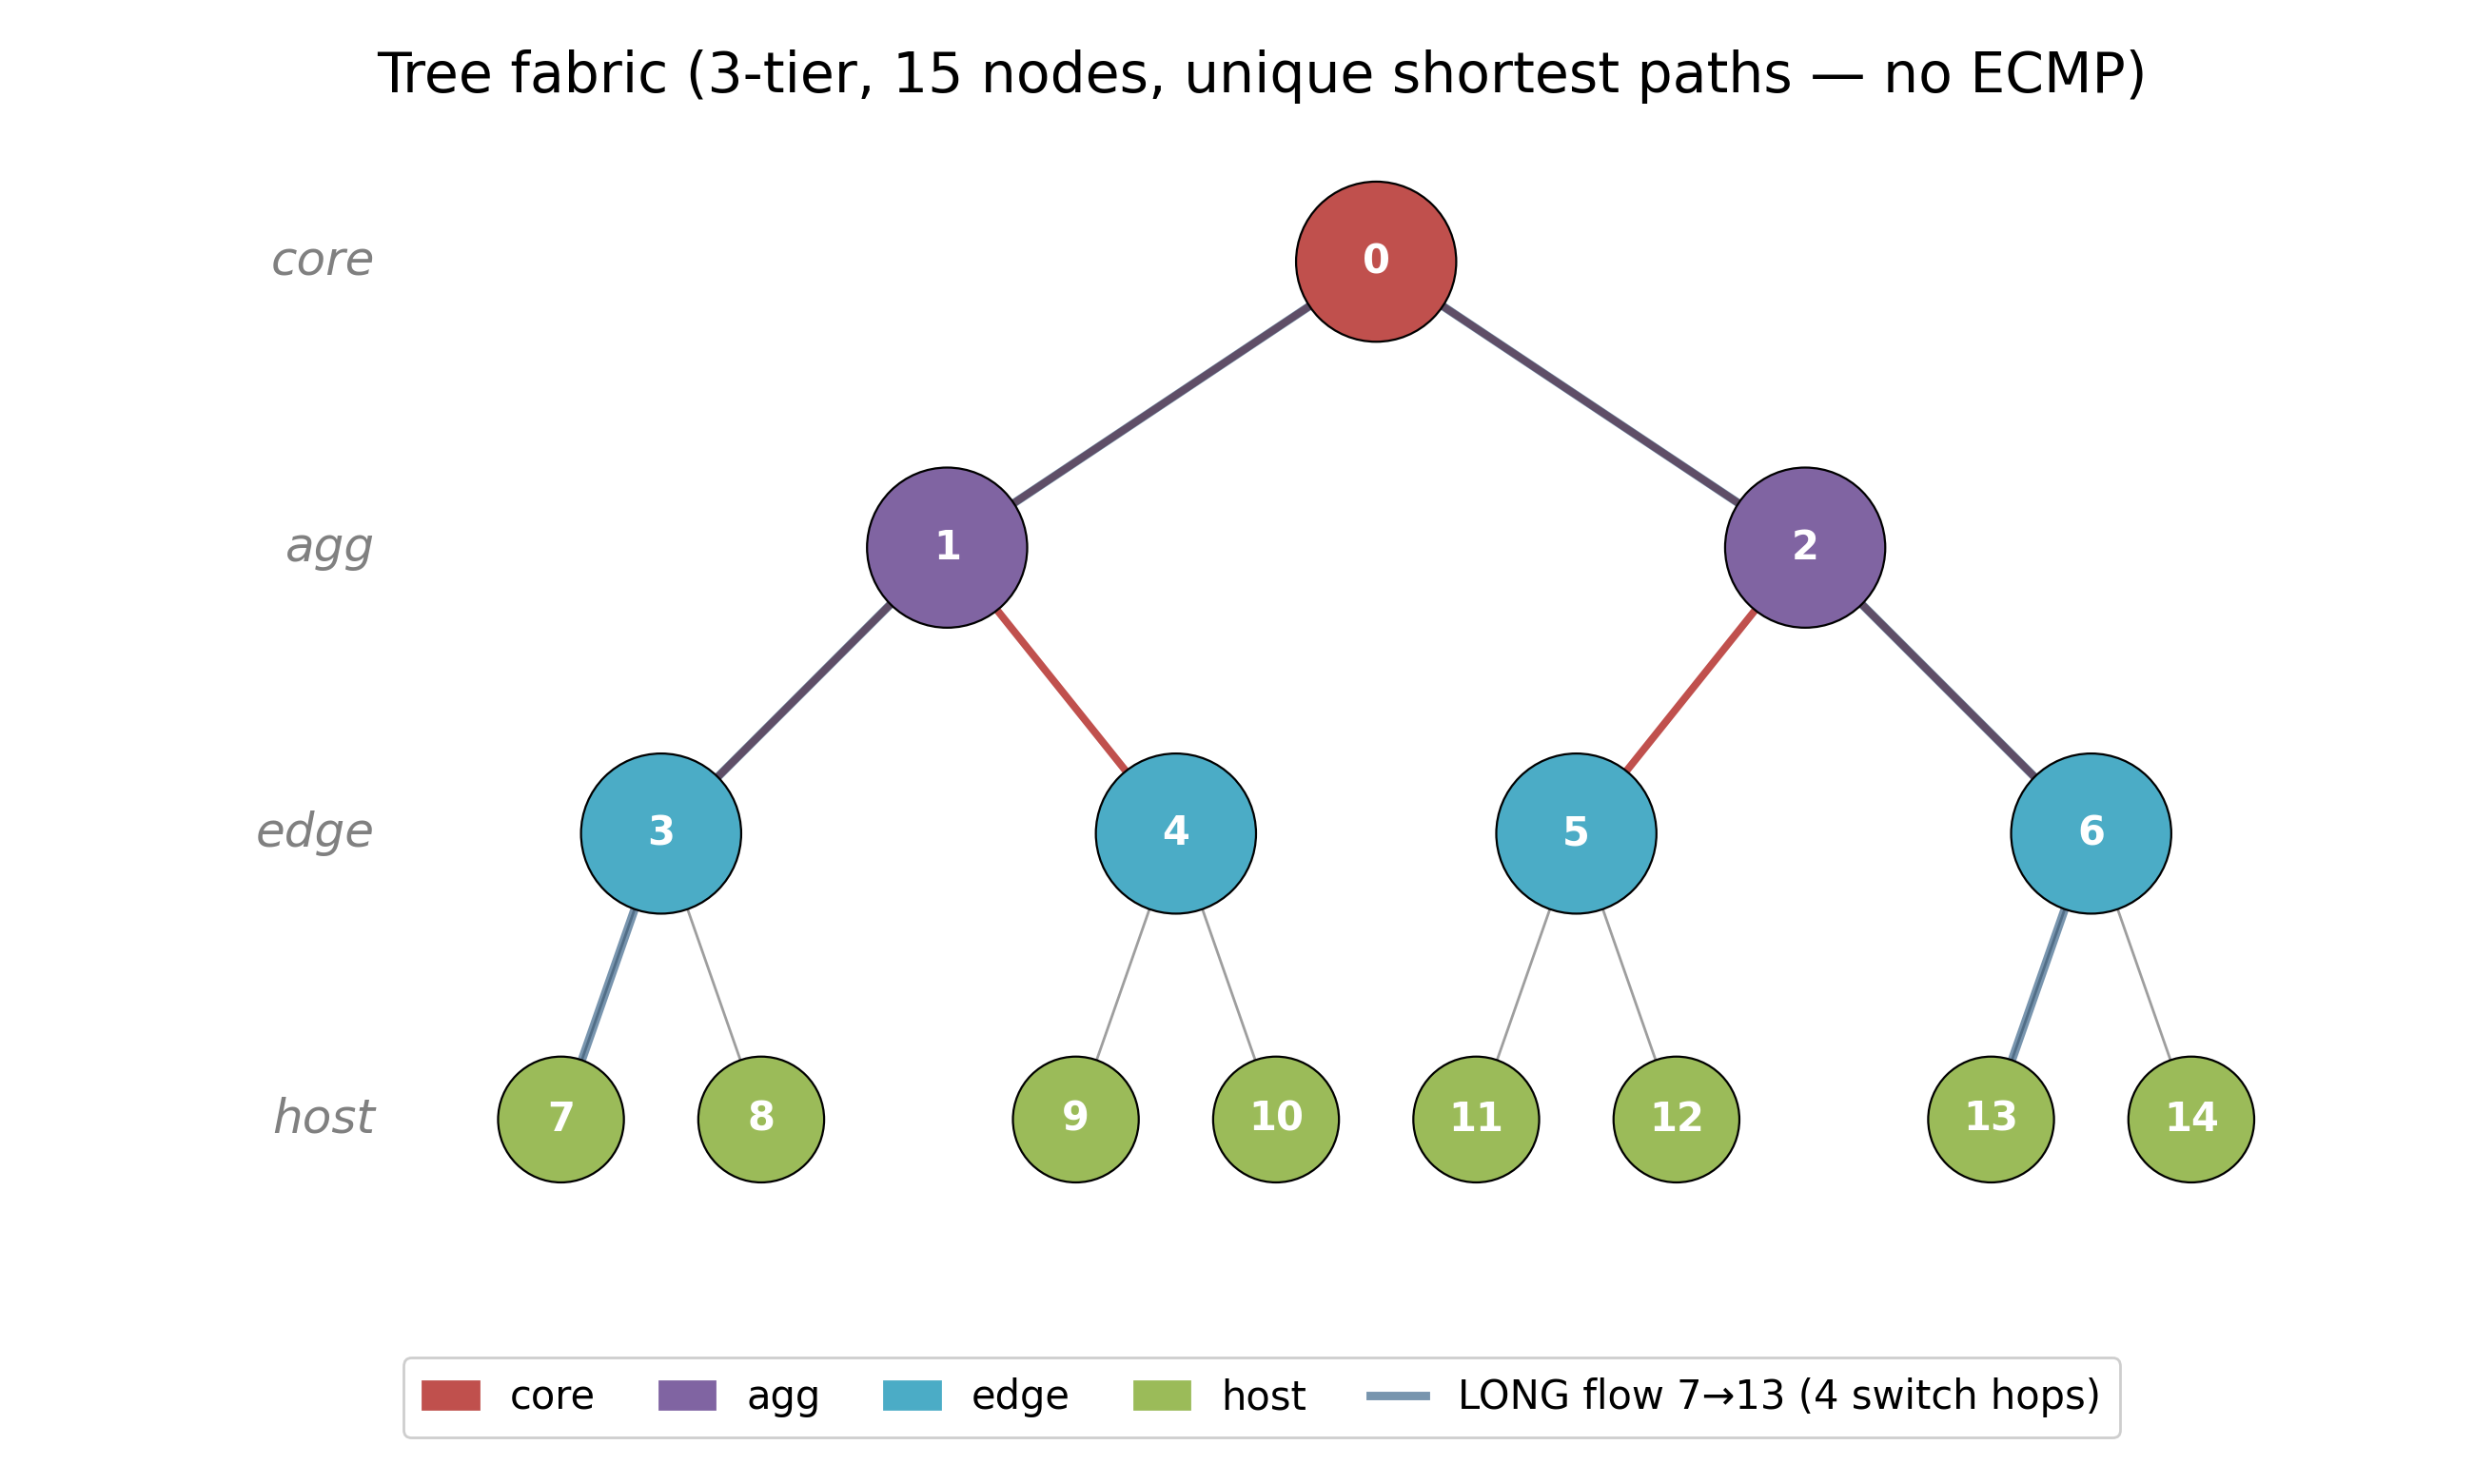
\includegraphics[width=0.86\textwidth]{fig_topo_tree.png}
\caption{Tree-fabric topology (3-tier, 15 nodes, unique shortest paths --- no ECMP). The
highlighted line is the long flow $7 \to 13$, which crosses four switches.}
\Description[3-tier tree fabric topology diagram]{3-tier tree fabric with 15 nodes: 1 core at
top, 2 aggregation switches, 4 edge switches, and 8 hosts at the bottom, with unique shortest
paths so no ECMP. A long flow from host 7 to host 13 is highlighted, crossing four switches.}
\label{fig:topo-tree}
\end{figure*}

\begin{figure*}[t]
\centering
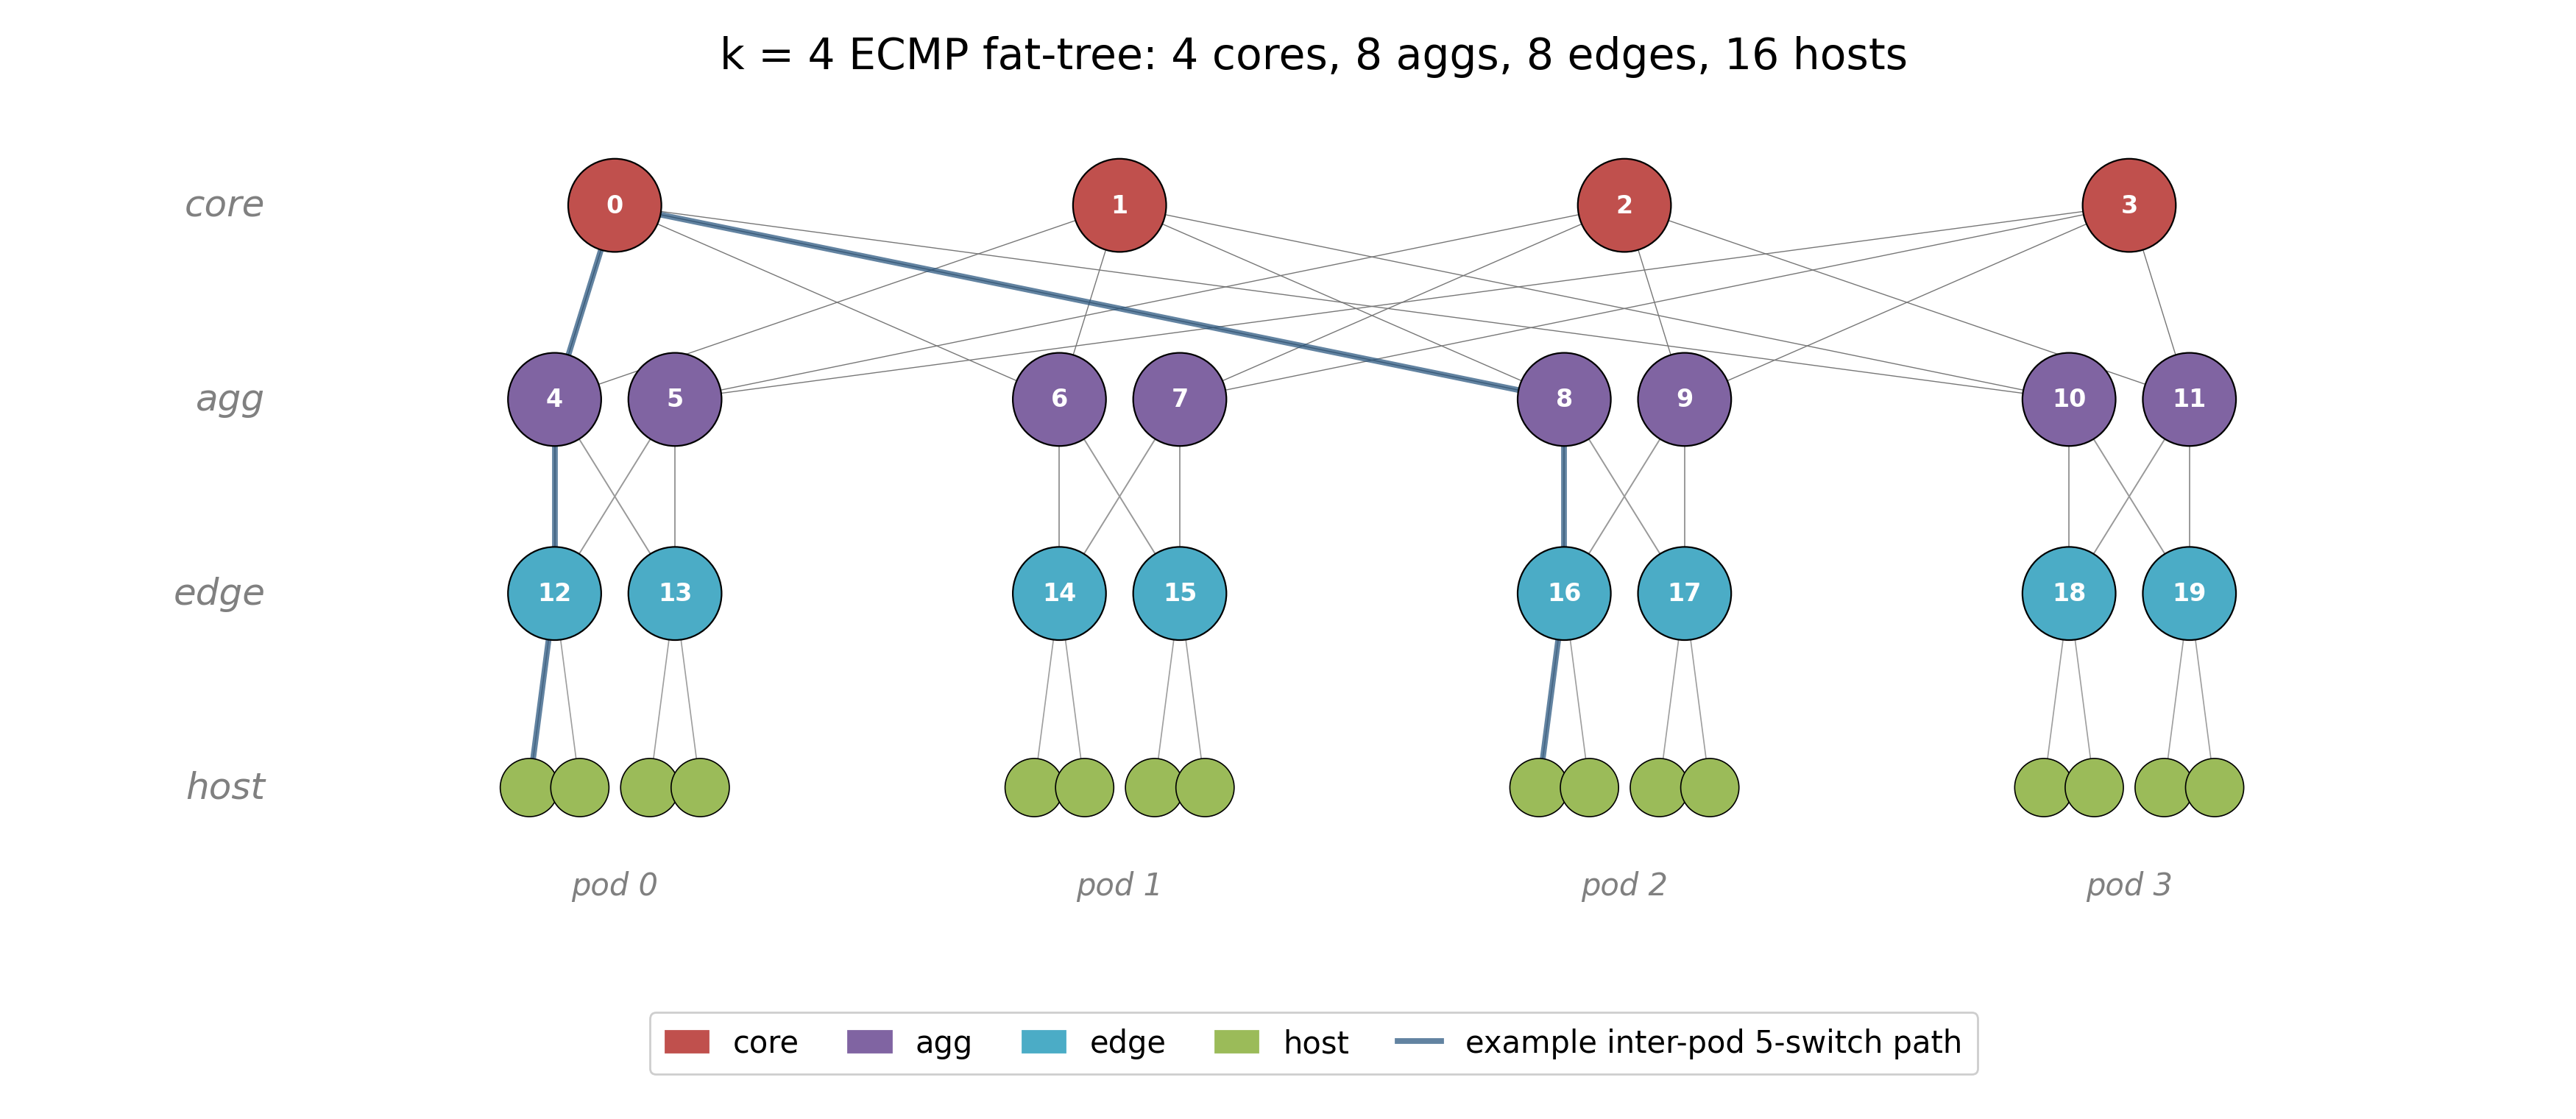
\includegraphics[width=0.96\textwidth]{fig_topo_fattree.png}
\caption{Canonical $k = 4$ ECMP fat-tree (4 cores, 8 aggs, 8 edges, 16 hosts in 4 pods). The
highlighted line is a representative inter-pod 5-switch path.}
\Description[k=4 ECMP fat-tree topology diagram]{Canonical k=4 fat-tree with 4 cores at top, 8
aggregation switches, 8 edge switches, and 16 hosts arranged in 4 pods of 4 hosts each. All
cores connect to all pods via the standard fat-tree pattern. A representative inter-pod
5-switch path is highlighted.}
\label{fig:topo-ft}
\end{figure*}

\paragraph{Tree fabric (3-tier, no ECMP).} A 3-tier tree with unique shortest paths (15 nodes;
25 Gbps inter-switch, 100 Gbps host; Figure~\ref{fig:topo-tree}). Stock penalty
$1.36\times$, \hpccfs $\mathbf{1.003\times}$, PFC $= 0$.

\paragraph{$k = 4$ fat-tree (with ECMP).} The canonical fat-tree (20 switches + 16 hosts; 48
links; Figure~\ref{fig:topo-ft}) with the simulator's hash-based ECMP routing.
Workload: 4 inter-pod flows (5-switch paths) plus 4 intra-pod different-edge flows (3-switch
paths). We report two distinct quantities. (i) The \emph{oracle-normalized penalty} --- mean
long-path slowdown divided by mean short-path slowdown, each measured against the max-min oracle
--- which removes the effect of ECMP load placement: stock $1.34\times$, \hpccfs
$\mathbf{1.001\times}$ (every contended flow lands at its oracle FCT). (ii) The \emph{raw}
long/short FCT ratio, which under HPCC-FS is still ${\sim}1.32\times$ --- but this residual is
\emph{not} CC unfairness: ECMP hashes some flows onto under-loaded cores so they finish early,
inflating the raw ratio independently of the congestion controller. PFC $= 0$ for both schemes.
The point is that, once ECMP load placement is normalized away, HPCC-FS removes the
multi-bottleneck penalty; the path-min fair-rate aggregation is path-invariant, so ECMP requires
no design changes.

\subsection{Robustness across asymmetric workloads}

\begin{figure}[t]
\centering
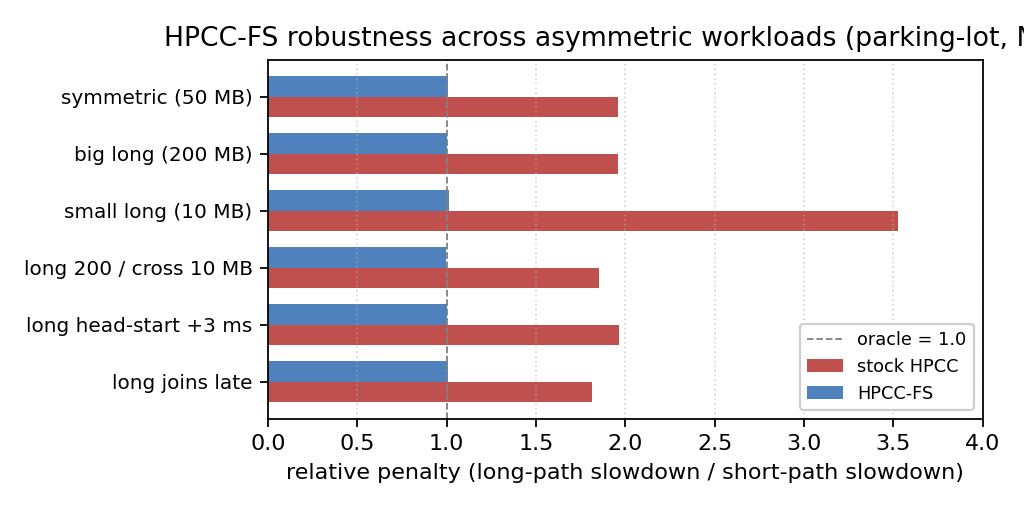
\includegraphics[width=\columnwidth]{fig_robustness.png}
\caption{Robustness across asymmetric-size and staggered-start variants at $N=4$. \hpccfs is
within $1.0 \pm 0.012$ across all six scenarios, including the small-long worst case where
stock reaches $3.53\times$.}
\Description[Horizontal bar chart of penalty across six workload variants]{Horizontal bars
comparing stock HPCC and HPCC-FS relative penalty across six asymmetric-size and staggered-start
scenarios at N=4. Stock bars range from 1.81x to 3.53x. HPCC-FS bars are clustered near 1.0
across all scenarios. A dashed vertical line at 1.0 marks the max-min oracle.}
\label{fig:robustness}
\end{figure}

Across six perturbations (Figure~\ref{fig:robustness}), \hpccfs holds within $1.0 \pm 0.012$.
The worst stock case (small multi-bottleneck flow, $3.53\times$ penalty) drops to $1.012\times$.

\subsection{Ablation: rate-only is necessary}
\label{sec:ablation}

\hpccfs runs rate-only in FS mode --- the per-flow window cap is disabled (\S\ref{sec:design}).
Table~\ref{tab:window} ablates this: re-enabling the window cap in FS mode degrades the penalty to
$1.5$--$2.5\times$, \emph{worsening with path length} (at $N=4$ it is worse than stock HPCC). The
cause is that \texttt{var\_win} sizes the window from the NIC line rate, not the smaller multi-hop
bottleneck path, so the long flow is window-bound below its fair rate. Disabling the cap is thus a
necessary part of the design, not an incidental change; the switch's RCP rate already keeps queues
bounded (zero PFC, \S\ref{sec:queue}).

\begin{table}[t]
\caption{Window ablation: HPCC-FS rate-only (default) vs.\ with the per-flow window cap re-enabled.}
\label{tab:window}
\centering
\small
\begin{tabular}{rcc}
\toprule
$N$ & FS rate-only (default) & FS window-on \\
\midrule
2 & $\mathbf{1.003\times}$ & $1.50\times$ \\
3 & $\mathbf{1.003\times}$ & $2.00\times$ \\
4 & $\mathbf{1.005\times}$ & $2.49\times$ \\
\bottomrule
\end{tabular}
\end{table}

\subsection{Parameter sensitivity}
\label{sec:sensitivity}

A reasonable concern is that HPCC-FS's RCP gains are tuned to the benchmark. They are not: we use
the standard RCP defaults ($\alpha = 0.4$, $\beta = 0.226$) untouched. Sweeping each parameter
\emph{one at a time} at $N = 4$ on the equal-size parking-lot (others at default), the
penalty stays within $[1.004, 1.008]\times$ with zero PFC throughout:
$\alpha \in [0.2, 0.6]$ ($1.004$--$1.007\times$),
$\beta \in [0.1, 0.4]$ ($1.005\times$, flat),
the startup fraction $R_0/C \in [0.25, 1.0]$ ($1.004$--$1.008\times$; even $R_0 = C$ is PFC-free,
because the sender's \texttt{m\_minRate} start absorbs the first-interval burst, \S\ref{sec:design}),
and $\mathit{minRate} \in [100, 2000]$ Mb/s ($1.005\times$, flat). Within this benchmark family the
RCP parameters are not load-bearing; we do not claim the same insensitivity for arbitrary
topologies, joint sweeps, or heterogeneous link speeds, which remain future work.

\subsection{Queueing and PFC}
\label{sec:queue}

With the smoothed startup (\S\ref{sec:design}.2), \hpccfs produces \textbf{zero PFC events} on
every workload in the $N$-sweep and the robustness matrix. ECN marking remains; queue length is
bounded (peak ${\approx}120$ KB at $N=4$); no flow loss.

\subsection{Do-no-harm}

The HPCC algorithm-validation smoke configuration (\texttt{cc\_mode 3}, single-bottleneck
incast) passes all checks: 6/6 flows complete, 0 PFC, validation artifacts byte-identical to
pre-modification. The stock \texttt{cc\_mode 3} $N$-sweep is bit-identical to the pre-change
baseline. The HPCC-FS additions affect the \texttt{cc\_mode 3} path only by adding new code; no
existing function's output for existing inputs is altered.

\subsection{HPCC's home turf: competitive FCT, lower queue}
\label{sec:cost}

On contended flows \hpccfs uses RCP-style switch-computed rates rather than HPCC's per-hop
control, so a fair question is what this costs on \emph{single}-bottleneck workloads --- HPCC's
home turf. We measure the validated incast benchmark (3 senders $\to$ 1 receiver over a 25 Gbps
bottleneck; 12 flows, 100--400 KB), sweeping the sender's startup rate (short flows begin at the
startup rate and ramp until the first fair-rate ACK returns):

\begin{table}[t]
\caption{HPCC's home turf (single-bottleneck incast). HPCC-FS holds far less queue than HPCC at
every startup, and a moderate startup also matches or beats HPCC's FCT. The same startup leaves
the multi-bottleneck fairness headline unchanged ($1.003$--$1.004\times$, PFC $= 0$).}
\label{tab:hometurf}
\centering
\small
\begin{tabular}{lccc}
\toprule
 & mean FCT & tail FCT & peak queue \\
\midrule
HPCC & 258.6 $\mu$s & 459.8 $\mu$s & 143 KB \\
\hpccfs (startup 1 Gbps) & 297.5 $\mu$s & 490.3 $\mu$s & \textbf{64 KB} \\
\hpccfs (startup 5 Gbps) & 271.2 $\mu$s & 464.3 $\mu$s & \textbf{49 KB} \\
\hpccfs (startup 8 Gbps) & \textbf{242.0 $\mu$s} & \textbf{416.8 $\mu$s} & \textbf{38 KB} \\
\bottomrule
\end{tabular}
\end{table}

Two things stand out (Table~\ref{tab:hometurf}). First, \hpccfs holds \emph{far less queue} than
HPCC at \emph{every} startup ($38$--$64$ KB vs $143$ KB) --- RCP's $\beta q/d$ term drains queue
aggressively. Second, the only place HPCC leads is FCT at the conservative 1 Gbps startup
(${\sim}15\%$); raising the startup closes and then \emph{reverses} that gap --- at 8 Gbps \hpccfs
beats HPCC's mean FCT (242 vs 259 $\mu$s) at roughly one-quarter the queue, with zero PFC. The
startup is a clean knob (queue rises again only past the point where the aggregate startup rate
exceeds link capacity), and crucially it does \emph{not} disturb the multi-bottleneck headline:
at 8 Gbps the parking-lot penalty stays $1.003$--$1.004\times$ ($N\!=\!2,3,4$) with robustness
variants $1.002$--$1.009\times$, all PFC $= 0$ (\S\ref{sec:cost} reuses the same operating point
as the headline). So on the home-turf workloads we measured, \hpccfs's fairness fix comes at
\emph{little-to-no FCT cost and a queue benefit} --- not a trade-off.

We are careful not to overclaim: \hpccfs still lacks HPCC's per-hop, window-bounded reaction, so
on rapidly-varying or adversarial-microburst workloads (which we did not evaluate) HPCC's
precision may matter; recovering that while keeping the fairness fix is what the hybrid overlay
of \S\ref{sec:discussion} targets.

\subsection{Per-flow rate trace, before vs after}

\begin{figure*}[t]
\centering

\includegraphics[width=\textwidth]{fig_rate_trace.png}
\caption{Per-flow goodput at $N = 4$, stock HPCC (left) vs \hpccfs (right). Stock collapses the
long flow to ${\sim}0.4$ Gbps while cross flows hold ${\sim}23$ Gbps for 18 ms (winner-take-all).
\hpccfs converges all five flows to the max-min fair share (12.5 Gbps) within ${\sim}4$ ms.}
\Description[Per-flow goodput over time, two panels]{Two side-by-side line plots of per-flow
goodput (Gbps) vs time (ms) at N=4. Left panel (stock HPCC): the long multi-bottleneck flow is
flat near 0.4 Gbps from t=1 ms to 18 ms while four cross flows hold 23 Gbps; after t=19 ms the
long flow takes the pipe at 23 Gbps. Right panel (HPCC-FS): all five flows converge to about
12.5 Gbps within 4 ms and stay locked there for the duration of the contention. A dashed line
at 12.5 Gbps marks max-min fair share.}
\label{fig:rate-trace}
\end{figure*}

The before-vs-after rate trace (Figure~\ref{fig:rate-trace}) is the cleanest qualitative result.
Stock HPCC: the long flow collapses to ${\sim}0.4$ Gbps while the four cross flows hold
${\sim}23$ Gbps each for the full 18 ms contention; \hpccfs: all five flows converge to
${\sim}12.5$ Gbps within ${\sim}4$ ms and stay locked at fair share.

% ============================================================================
\section{Related Work}
\label{sec:related}
% ============================================================================

\paragraph{Datacenter transport.} A long line of datacenter congestion control trades buffering for
latency. DCTCP~\cite{alizadeh2010dctcp} reacts to ECN-marked standing queue; DCQCN~\cite{zhu2015dcqcn}
and TIMELY~\cite{mittal2015timely} bring rate-based control to lossless RDMA fabrics using ECN and
delay respectively; and Swift~\cite{kumar2020swift} shows a carefully engineered delay signal scales
to large fabrics. Receiver- and scheduling-driven designs such as Homa~\cite{montazeri2018homa} and
pFabric~\cite{alizadeh2013pfabric} instead prioritize short flows for low FCT. HPCC~\cite{li2019hpcc}
marked a shift toward \emph{in-network telemetry}: rather than infer congestion from a single scalar,
the sender reads exact per-hop link load and sizes its window precisely, and
On-Ramp~\cite{liu2021onramp} and PowerTCP~\cite{addanki2022powertcp} push the precise-signal philosophy
further. Across this line the optimization target is overwhelmingly single-bottleneck FCT, tail latency,
or queueing; \emph{fairness across multiple shared bottlenecks}---our focus---receives comparatively
little attention, and we show it is exactly where HPCC's otherwise-precise control breaks.

\paragraph{In-network telemetry.} INT~\cite{kim2015int} lets the data plane stamp per-hop state into
packets on programmable pipelines, and HPCC was among the first to drive congestion control directly
from it. The cost is header overhead, which later work minimizes: HPCC-PINT~\cite{yang2020pint}
compresses the per-hop record into a single probabilistic field, and Poseidon~\cite{wang2023poseidon}
restructures INT-based control for deployability on commodity hardware. \hpccfs continues this
minimal-telemetry direction but changes \emph{what} the field carries: not a raw load sample to be
interpreted by the sender, but an explicit fair \emph{rate} computed at the switch and min-aggregated
along the path---one 64-bit field, like PINT, yet a decision rather than a measurement.

\paragraph{Explicit-rate and switch-assisted control.} Having the switch compute and return a sending
rate is a classic idea. ATM ABR explicit-rate schemes such as ERICA~\cite{kalyanaraman2000erica}
computed a fair share per port decades ago; XCP~\cite{katabi2002xcp} decomposed switch feedback into
separate efficiency and fairness controllers; and RCP~\cite{dukkipati2008rcp} reduced this to a single
fair-rate scalar per link with no per-flow state, packet-stamped, with senders taking the path minimum.
RCP is the closest mechanism to ours: \hpccfs adopts its update rule but situates it as a \emph{minimal
fairness signal injected into an existing INT load-signaling system} rather than a standalone protocol,
keeping HPCC's single-rate sender and per-hop transport. ABC~\cite{goyal2020abc} argues, for wireless
links, that switches should compute the right control signal rather than expose raw load; we apply the
same philosophy with minimal departure from HPCC's datacenter design.

\paragraph{In-switch fairness.} A parallel line enforces fairness inside the switch via scheduling or
dropping. Fair queueing~\cite{demers1989fq} and Deficit Round Robin~\cite{shreedhar1995drr} give each
flow its own queue, while Core-Stateless Fair Queueing~\cite{stoica1998csfq} and Approximate Fair
Dropping~\cite{pan2003afd} approximate fair bandwidth shares \emph{without} per-flow queues---using a
single estimated fair rate and probabilistic dropping, the same stateless-per-flow spirit as RCP and
\hpccfs. Programmable schedulers such as PIFO~\cite{sivaraman2016pifo} and AIFO~\cite{yu2021aifo} make
rich scheduling policies realizable at line rate. \hpccfs differs in mechanism: rather than enforcing
fairness by per-packet queueing or dropping, it \emph{advertises} one fair rate per egress port and
lets rate-controlled RDMA senders converge to it---one scalar of egress state, no per-flow tracking and
no extra queues.

\paragraph{Programmable-switch feasibility.} Reconfigurable match-action pipelines~\cite{bosshart2013rmt}
and P4~\cite{bosshart2014p4} make the per-port computation \hpccfs needs---an EWMA of egress load, a
multiply--add rate update, and stamping one header field---implementable on the same class of
programmable switches that HPCC's INT and Bolt~\cite{arslan2023bolt} already assume.

\paragraph{Closely related switch-assisted DC schemes.} Bolt~\cite{arslan2023bolt} targets HPCC's
latency limits with Sub-RTT Control, Proactive Ramp-Up, and Supply Matching on programmable switches,
reporting ${\sim}3\times$ FCT improvement and ${\sim}80\%$ tail-latency reduction over HPCC at
400~Gbps; it focuses on tail latency and ramp-up rather than multi-bottleneck max-min fairness and
keeps richer per-flow switch state than our single scalar per port. A direct head-to-head on the
multi-bottleneck workload of \S\ref{sec:bg} would clarify how Bolt's per-flow window adjustments
interact with the dynamics we characterize. Annulus~\cite{saeed2020annulus} uses a dual-control-loop
design for traffic aggregates mixing WAN and datacenter flows---largely orthogonal to intra-DC
multi-bottleneck fairness within a single class.

\paragraph{Fairness foundations.} Max-min fairness and the progressive-filling characterization we use
as our oracle are classical~\cite{bertsekas1992data}, and the parking-lot topology is a standard stress
test for multi-bottleneck rate allocation. Our contribution is not a new fairness definition but the
diagnosis that HPCC cannot realize this well-understood objective from sender-visible INT alone, and
the demonstration that a single switch-computed fair rate restores it.

% ============================================================================
\section{Discussion}
\label{sec:discussion}
% ============================================================================

\paragraph{Relation to HPCC, and a hybrid path.} \hpccfs is best understood not as a tweak to
HPCC's control law but as a demonstration of \emph{where} the multi-bottleneck fix must live: a
fair-share signal computed at the switch, which we instantiate with RCP. On contended flows it
therefore replaces HPCC's window-bounded, per-hop-INT control with an RCP-style rate, and inherits
RCP's character --- fair and low-queue, but without HPCC's aggressive single-flow precision
(\S\ref{sec:cost}). The natural way to keep both is a \emph{hybrid overlay}: run HPCC unchanged on
every flow and use the switch's fair rate only as a per-flow \emph{ceiling},
$\mathit{rate} = \min(\mathit{rate}_{\mathrm{HPCC}}, \mathit{fairRate})$, so dominant flows are
capped to their fair share (and yield bandwidth that HPCC's own increase gives to the starved
flow) while HPCC's window and reaction are preserved. The open obstacle is the window--path
mismatch behind our rate-only choice (\S\ref{sec:design}): HPCC's window is sized for the NIC, not
the multi-hop bottleneck path, so a victim flow may stay window-bound below fair even after the
ceiling frees bandwidth --- the overlay likely needs a path-aware window. We leave this hybrid,
which would retain HPCC's precision \emph{and} its fairness, to future work.

\paragraph{INT hop limit and the non-monotonic flip.} The $\texttt{maxHop} = 5$ limit in the
INT-header layout is the source of the non-monotonic regime change in stock HPCC: paths longer
than five switches overflow the INT record and the rate-control input is corrupted. \hpccfs
sidesteps this because its wire format carries one field independent of hop count, and our
$N = 5, 6$ measurements (\S\ref{sec:eval}) confirm it remains at penalty ${\approx}1.0\times$
in that regime.

\paragraph{Mixed-size workloads.} In a preliminary test on the parking-lot under a Web-Search
size distribution (30 flows, 483~B to 9.6~MB), \hpccfs reduces multi-bottleneck flow mean
slowdown by ${\sim}15\%$ but increases short-path mean slowdown by ${\sim}45\%$. This is correct
max-min behaviour --- stock HPCC's starvation of the long flow was inflating cross-link headroom
that short flows benefited from --- but it surfaces a workload-engineering question that max-min
alone does not resolve. A defensible mixed-size evaluation needs per-class targets and is
application-dependent; we leave it to follow-on work.

\paragraph{Scaling to larger fat-trees.} The fat-tree generator runs at $k = 6$ (45 switches, 36
hosts) and $k = 8$ (80 switches, 64 hosts). At larger $k$ the fabric has $(k/2)^2$ cores, so
inter-pod flows spread across uncongested core paths and persistent contention does not
materialize for our scaling workload --- both stock and \hpccfs show penalty ${<}1$, an ECMP
load-distribution effect. \hpccfs adds no overhead in this regime (0 PFC across all six runs).
A workload designed to saturate larger fabrics with guaranteed inter-pod contention is open
future work.

\paragraph{Heterogeneous link speeds.} Our parking lot has uniform 25 Gbps bottlenecks. Mixed
link speeds may interact with RCP's $\alpha(C-y)$ term in ways the symmetric case does not
exercise. RCP itself is known to handle heterogeneity gracefully; we expect the same for
\hpccfs but have not verified.

\paragraph{Multi-path / ECMP.} \S\ref{sec:eval} shows \hpccfs works under ECMP on a $k=4$
fat-tree with hash-based path selection --- the path-min fair-rate aggregation is itself
path-invariant. ECMP load imbalance does produce per-flow FCT spread, but this is a routing
issue, not a CC issue.

\paragraph{Hardware feasibility.} RCP's update is a single per-port floating-point or
fixed-point step with three multiplies and an add; it is well within the budget of programmable
switches. The min-aggregation per packet is a 64-bit compare and conditional write.

\paragraph{Limitations.} Three topology families (parking-lot, tree-fabric, $k = 4{-}8$
fat-tree) and one in-sim baseline (HPCC-PINT); no head-to-head with hardware-assisted designs
such as Bolt or PowerTCP, which would require re-implementing them in this simulator; no testbed
measurements; convergence is a few ms (not one RTT, \S\ref{sec:design}); and the ECMP evaluation
is a small controlled workload, not a realistic mixed-size + ECMP combination. We did, however,
verify that the result is insensitive to the RCP parameters (\S\ref{sec:sensitivity}), so the
absence of tuning is not a hidden confound.

% ============================================================================
\section{Conclusion}
% ============================================================================

We have shown that HPCC's load-signaling INT design has a structural fairness failure in
multi-bottleneck workloads --- a real, robust, RTT-independent winner-take-all collapse with
${\sim}2\times$ FCT penalty for the multi-bottleneck flow, up to $3.5\times$ for small such
flows. No sender-side correction we attempted (across five representative variants) closes the
gap, because at the $\eta$-hold equilibrium additive nudges are too slow and the sender cannot
compute its fair share without knowing the link's flow count. A minimal extension that
suffices on our benchmarks is \textbf{one fair-rate field} in a new INT mode plus \textbf{one
scalar of state per switch port} (and, in our prototype, disabling the per-flow window cap in FS
mode --- see Section~\ref{sec:design}). The resulting protocol, \hpccfs, achieves max-min fairness
with penalty $1.005\times$ and zero PFC at $N = 4$ across all workloads we tested, converging in a
few milliseconds independent of path length, while leaving the original HPCC code path unchanged.

\bibliographystyle{ACM-Reference-Format}
\bibliography{paper}

\end{document}
